% =====================================================================
%  K-MER EVENT — Project Report (LaTeX)
%  Adapté du modèle ICTU (style et entête conservés).
%
%  COMPILATION :
%     pdflatex K-MER-EVENT-Report.tex
%     pdflatex K-MER-EVENT-Report.tex   (2x pour la table des matières / liste des figures)
%
%  PAQUETS REQUIS (tous inclus dans une distribution TeX Live / MiKTeX complète) :
%     tikz, pgfplots, pgf-umlsd, tcolorbox, booktabs, hyperref, fancyhdr, titlesec
%
%  IMAGES À FOURNIR :
%     - ictu_logo.png        (logo de l'université ; sinon un cadre de remplacement s'affiche)
%     - Les CAPTURES D'ÉCRAN de l'application et les graphiques de sondage
%       (voir les encadrés "[CAPTURE D'ÉCRAN À INSÉRER]").
%
%  À PERSONNALISER (cherchez "TODO") : votre nom, votre matricule, vos données de sondage.
% =====================================================================

\documentclass[12pt,a4paper]{report}

\usepackage[utf8]{inputenc}
\usepackage[T1]{fontenc}
\usepackage[english]{babel}
\usepackage[a4paper,margin=2.5cm]{geometry}
\usepackage{graphicx}
\usepackage{float}
\usepackage{xcolor}
\usepackage{tikz}
\usetikzlibrary{shapes.geometric,shapes.multipart,arrows.meta,positioning,fit,calc}
\usepackage{pgfplots}
\pgfplotsset{compat=1.17}
\usepackage{pgf-umlsd}
\usepackage{tcolorbox}
\usepackage{booktabs}
\usepackage{longtable}
\usepackage{array}
\usepackage{enumitem}
\usepackage{setspace}
\usepackage{titlesec}
\usepackage{fancyhdr}
\usepackage[hidelinks]{hyperref}

\onehalfspacing

% ---- Couleur d'accent de la plateforme (terracotta / ocre) ----
\definecolor{kmerwarm}{HTML}{C2410C}
\definecolor{kmerteal}{HTML}{0F766E}

% ---- En-têtes ----
\pagestyle{fancy}
\fancyhf{}
\fancyfoot[C]{\thepage}
\renewcommand{\headrulewidth}{0pt}

% ---- Commande : encadré de remplacement pour les captures d'écran ----
\newcommand{\screenshot}[1]{%
  \begin{center}
  \setlength{\fboxsep}{10pt}%
  \fbox{\parbox[c][4.2cm][c]{0.8\textwidth}{\centering
      \textbf{\color{red}[CAPTURE D'ÉCRAN À INSÉRER]}\\[6pt]
      \normalfont #1}}%
  \end{center}}

% ---- Commande : logo avec repli si l'image manque ----
\newcommand{\logoblock}{%
  \IfFileExists{ictu_logo.png}%
    {\includegraphics[width=3.8cm]{ictu_logo.png}}%
    {\setlength{\fboxsep}{8pt}\fbox{\parbox[c][3cm][c]{3.8cm}{\centering Logo université\\\texttt{ictu\_logo.png}}}}}

% ---- Styles TikZ pour les organigrammes ----
\tikzset{
  startstop/.style={rectangle, rounded corners, minimum width=2.6cm, minimum height=0.8cm, align=center, draw=black, fill=kmerteal!10},
  process/.style={rectangle, minimum width=2.6cm, minimum height=0.8cm, align=center, text width=2.8cm, draw=black, fill=white},
  decision/.style={diamond, aspect=2, minimum width=2.4cm, align=center, text width=2.2cm, draw=black, fill=kmerwarm!12, inner sep=1pt},
  io/.style={trapezium, trapezium left angle=70, trapezium right angle=110, minimum width=2cm, align=center, draw=black, fill=kmerteal!8},
  flow/.style={-{Latex[length=2mm]}},
  uc/.style={ellipse, draw=black, align=center, minimum width=2.6cm, minimum height=0.9cm, text width=2.6cm, font=\footnotesize, fill=white},
  actor/.style={rectangle, rounded corners, draw=black, align=center, minimum width=1.8cm, minimum height=0.9cm, fill=kmerwarm!12, font=\bfseries\small},
  classbox/.style={rectangle split, rectangle split parts=3, draw=black, fill=white, text width=3.4cm, align=left, font=\footnotesize, rectangle split part align=left},
  entity/.style={rectangle split, rectangle split parts=2, draw=black, fill=kmerteal!6, text width=3.2cm, align=left, font=\footnotesize, rectangle split part align=left},
}

% =====================================================================
\begin{document}
\pagenumbering{roman}

% ----------------------------- PAGE DE TITRE -----------------------------
\begin{titlepage}
\centering
\logoblock\par
\vspace{0.8cm}
{\large\bfseries THE INFORMATION, COMMUNICATION AND TECHNOLOGY\\
UNIVERSITY (ICTU), Yaound\'e, Cameroon.\par}
\vspace{0.8cm}

\begin{tcolorbox}[colback=kmerwarm!12,colframe=kmerwarm,boxrule=1pt,arc=4pt]
\centering\bfseries\large
DESIGN AND IMPLEMENTATION OF AN ONLINE EVENT BOOKING AND TICKETING PLATFORM
TO STREAMLINE EVENT DISCOVERY (K-MER EVENT)
\end{tcolorbox}

\vspace{0.8cm}
{\large\bfseries PROJECT REPORT\par}
\vspace{0.4cm}
A dissertation submitted in partial fulfilment of the requirement for the award of a\par
\vspace{0.2cm}
{\large\bfseries BACHELOR OF SCIENCE IN SOFTWARE ENGINEERING (BSc)\par}
\vspace{0.8cm}
By\par
\vspace{0.2cm}
{\large\bfseries NDONGO PHAREL\par}     % TODO: votre nom complet
{\bfseries ICTU20XXXXXX\par}            % TODO: votre matricule
\vspace{0.6cm}
{\bfseries Faculty of Information and Communication Technology\par}
\vspace{0.3cm}
{\bfseries MAJOR IN SOFTWARE ENGINEERING\par}
\vspace{0.8cm}
Supervised by:\par
{\bfseries Mr. ATANGANA\par}
\vfill
\begin{tcolorbox}[colback=kmerwarm!18,colframe=kmerwarm!18,width=0.6\textwidth]
\centering\bfseries Academic year 2025-2026
\end{tcolorbox}
\end{titlepage}

% ----------------------------- DECLARATION -----------------------------
\chapter*{DECLARATION}
\addcontentsline{toc}{chapter}{DECLARATION}
I declare that the work entitled \textbf{``DESIGN AND IMPLEMENTATION OF AN ONLINE EVENT
BOOKING AND TICKETING PLATFORM TO STREAMLINE EVENT DISCOVERY (K-MER EVENT)''} is my
original work, conceived and presented in partial fulfilment of the requirement for the
award of the degree of a Bachelor of Science in Software Engineering at the Information,
Communication, and Technology (ICT) University. This work has not been submitted for any
degree or examination in any other university, and all the sources I have used or quoted
have been indicated and acknowledged as complete references.

\vspace{1.5cm}
\noindent Name: \textbf{NDONGO PHAREL}\\[2pt]      % TODO
Registration Number: \textbf{ICTU20XXXXXX}          % TODO

\vspace{1.2cm}
\noindent Signature: \underline{\hspace{6cm}}

\vspace{1.0cm}
\noindent Date: \underline{\hspace{6cm}}

% ----------------------------- CERTIFICATION -----------------------------
\chapter*{CERTIFICATION}
\addcontentsline{toc}{chapter}{CERTIFICATION}
This project titled \textbf{``DESIGN AND IMPLEMENTATION OF AN ONLINE EVENT BOOKING AND
TICKETING PLATFORM TO STREAMLINE EVENT DISCOVERY (K-MER EVENT)''} is at this moment
approved as a credible study in Software Engineering carried out by NDONGO PHAREL
(ICTU20XXXXXX) a student at the ICT University in a satisfactory manner to warrant its
acceptance as a prerequisite to the degree of Bachelor of Science in Software Engineering
for which it has been submitted.

\vspace{1.2cm}
\noindent Mr. ATANGANA\\
Lecturer, the ICT University, Cameroon

\vspace{1.0cm}
\noindent Signature: \underline{\hspace{6cm}}

\vspace{1.0cm}
\noindent Date: \underline{\hspace{6cm}}

% ----------------------------- DEDICATION -----------------------------
\chapter*{DEDICATION}
\addcontentsline{toc}{chapter}{DEDICATION}
This project is dedicated to my parents, whose sacrifices and belief in my abilities have
driven me to achieve my goals. To my lecturers, whose guidance and wisdom have shaped my
academic journey, and to every event organizer and attendee in Cameroon who believes in
the power of technology to bring people together.

% ----------------------------- ACKNOWLEDGEMENT -----------------------------
\chapter*{ACKNOWLEDGEMENT}
\addcontentsline{toc}{chapter}{ACKNOWLEDGEMENT}
I would like to express my sincere gratitude to:\par
\textbf{God almighty} for the strength, guidance, protection, and wisdom to carry on this
task from start to completion.\par
\textbf{Mr. ATANGANA}, my supervisor, for the diligent assistance, recommendations, and
adjustments which helped me remain focused and determined in carrying out this work.\par
\textbf{My parents and siblings} for their support during this academic journey, and my
friends who helped make this endeavour a success.

% ----------------------------- FACULTY APPROVAL -----------------------------
\chapter*{FACULTY APPROVAL}
\addcontentsline{toc}{chapter}{FACULTY APPROVAL}
This project titled \textbf{``DESIGN AND IMPLEMENTATION OF AN ONLINE EVENT BOOKING AND
TICKETING PLATFORM TO STREAMLINE EVENT DISCOVERY (K-MER EVENT)''}, is at this moment
approved as a credible study in Software Engineering carried out by NDONGO PHAREL
(ICTU20XXXXXX), a student at the ICT University, in a satisfactory manner to warrant its
acceptance as a prerequisite to the degree of Bachelor of Science in Software Engineering
for which it has been submitted.

\vspace{1cm}
\noindent Approved by

\vspace{0.8cm}
\noindent Signature: \underline{\hspace{6cm}}\\[4pt]
Date: \underline{\hspace{6cm}}\\
Mr. ATANGANA --- Supervisor

\vspace{1.2cm}
\noindent Signature: \underline{\hspace{6cm}}\\[4pt]
Date: \underline{\hspace{6cm}}\\
Interim Dean

% ----------------------------- ABSTRACT -----------------------------
\chapter*{ABSTRACT}
\addcontentsline{toc}{chapter}{ABSTRACT}
The rapid growth of cultural, musical and professional events in Cameroon has created a
strong need for a reliable, digital way to discover events and purchase tickets. The
primary objective of this research is to design and implement \textbf{K-MER EVENT}, a
centralized web platform that streamlines event discovery, booking and ticketing, while
giving organizers the tools to publish and manage their events. The problem addressed is
the inefficiency, insecurity and informality of current event ticketing, which still
relies on physical tickets, word of mouth and cash, leading to fraud, long queues and poor
visibility for organizers.

A comprehensive methodology was employed, involving a critical review of existing ticketing
platforms, user requirement analysis, system design and iterative development. The
development followed the \textbf{Model--View--Controller (MVC)} pattern, using
\textbf{React} for the client interface, \textbf{Node.js/Express} with \textbf{Sequelize}
and \textbf{MySQL} for the server side, \textbf{JWT} for role-based authentication, and
\textbf{Socket.IO} for real-time updates. Core features include role-based accounts
(attendee, organizer, admin), advanced event discovery and filtering, a shopping cart and
checkout, \textbf{PDF tickets with QR codes}, \textbf{QR check-in at the entrance}, an
\textbf{automatic waitlist} with e-mail notifications, automatic \textbf{geolocation} with a
\textbf{satellite map} on the event page, favorites and WhatsApp sharing.

The findings show that K-MER EVENT significantly improves the efficiency and security of the
ticketing process: QR tickets cannot be duplicated, organizers gain real-time statistics,
and attendees can find and book events in under a minute. The platform demonstrates the
potential of modern web technologies to transform the event industry in Cameroon. Future
work includes integrating Mobile Money (MTN/Orange) and a native mobile application.

\vspace{4pt}
\noindent\textbf{Keywords:} K-MER EVENT, event booking, QR ticketing, real-time web
application, geolocation, waitlist, Cameroon, MVC.

% ----------------------------- TOC / LISTS -----------------------------
\tableofcontents
\listoffigures
\addcontentsline{toc}{chapter}{List of Figures}
\listoftables
\addcontentsline{toc}{chapter}{List of Tables}

% ---- Acronyms ----
\chapter*{List of Acronyms and Abbreviations}
\addcontentsline{toc}{chapter}{List of Acronyms and Abbreviations}
\begin{description}[leftmargin=3.2cm,style=nextline,labelwidth=3cm]
  \item[API] Application Programming Interface
  \item[CRUD] Create, Read, Update, Delete
  \item[CORS] Cross-Origin Resource Sharing
  \item[CSS] Cascading Style Sheet
  \item[ER Diagram] Entity Relationship Diagram
  \item[HTML] Hyper Text Markup Language
  \item[JWT] JSON Web Token
  \item[MVC] Model View Controller
  \item[ORM] Object Relational Mapping
  \item[PDF] Portable Document Format
  \item[QR] Quick Response (code)
  \item[RBAC] Role-Based Access Control
  \item[RDBMS] Relational Database Management System
  \item[REST] Representational State Transfer
  \item[SDLC] Software Development Life Cycle
  \item[SPA] Single Page Application
  \item[UAT] User Acceptance Testing
  \item[UI/UX] User Interface / User Experience
  \item[UML] Unified Modelling Language
\end{description}

% =====================================================================
\clearpage
\pagenumbering{arabic}

% ============================ CHAPTER 1 ==============================
\chapter{INTRODUCTION}

\section{Introduction}
The events industry in Cameroon --- concerts, festivals, conferences, cultural nights and
sporting events --- is growing rapidly. Yet the way people discover events and obtain
tickets remains largely informal: physical tickets, posters, social-media announcements and
cash payments at the gate. This creates fraud, counterfeit tickets, long queues and poor
visibility for organizers. \textbf{K-MER EVENT} is a centralized web platform designed to
solve these problems by connecting attendees with organizers and delivering secure
\textbf{QR-code tickets}, real-time availability, and a modern, intuitive interface.

The platform allows attendees to search and filter events by city, category, date and
price, add tickets to a cart, check out, and instantly receive a downloadable PDF ticket
with a unique QR code. Organizers can publish and manage their events, set capacities and
prices, and validate tickets at the entrance through QR check-in. Administrators oversee the
whole platform: validating events, managing users and monitoring activity through an
analytics dashboard.

\section{Background to the Problem}
The advent of the internet has transformed many sectors, including entertainment and event
management. Globally, platforms such as Eventbrite, Ticketmaster and Universe have digitized
ticketing. In Cameroon and much of Central Africa, however, event ticketing is still mostly
manual. Attendees rely on word of mouth and physical points of sale, while organizers
struggle with capacity management, revenue tracking and fraud prevention. The lack of a
trusted, centralized and locally adapted platform is a persistent challenge.

\section{Problem Statement}
The main problems K-MER EVENT aims to address are:
\begin{enumerate}
  \item \textbf{Insecure ticketing:} physical and printed tickets are easily duplicated or
        forged, causing revenue loss and access-control problems at the entrance.
  \item \textbf{Poor discoverability:} attendees have no single place to discover upcoming
        events, compare prices, see locations, or know how many seats remain.
  \item \textbf{Manual capacity management:} organizers cannot track sales in real time, and
        sold-out events offer no mechanism to capture interested attendees.
  \item \textbf{Lack of trust and visibility:} without verified organizers, official event
        pages and confirmations, attendees hesitate to pay in advance.
\end{enumerate}

\section{Objectives}
\subsection{General Objective}
To design and implement K-MER EVENT, a centralized web platform that streamlines event
discovery, booking and secure ticketing, while enhancing accessibility and trust for both
attendees and organizers.

\subsection{Specific Objectives}
\begin{enumerate}
  \item To develop a secure, role-based web application (attendee, organizer, admin) with
        JWT authentication.
  \item To implement secure ticketing using downloadable PDF tickets with unique QR codes and
        QR check-in at the entrance.
  \item To provide advanced event discovery (search, filters, favorites, WhatsApp sharing)
        and a satellite-map location on each event page.
  \item To implement real-time updates (Socket.IO) and an automatic waitlist with e-mail
        notifications when seats free up.
\end{enumerate}

\section{Research Questions}
\begin{enumerate}
  \item How does K-MER EVENT simplify the event discovery and booking process for attendees?
  \item How does QR-based ticketing and check-in improve security and access control?
  \item In what ways does the platform help organizers manage capacity and track sales in
        real time?
  \item What impact does the platform have on the accessibility and trust of event ticketing
        in Cameroon?
\end{enumerate}

\section{Scope of Research}
\subsection{Technological Scope}
\begin{itemize}
  \item \textbf{User interface and experience:} a responsive Single Page Application with a
        readable light/dark theme.
  \item \textbf{Backend:} a secure REST API managing accounts, events, carts, bookings,
        ticketing and check-in.
  \item \textbf{Search and discovery:} filtering by city, category, price, date and favorites.
  \item \textbf{Real-time tools:} live event updates via WebSocket.
  \item \textbf{Geolocation:} automatic geocoding of the venue and a satellite map.
  \item \textbf{Security:} role-based access control and tamper-proof QR tickets.
\end{itemize}

\subsection{Regional Coverage}
The platform initially targets major Cameroonian cities (Yaound\'e, Douala) with the
intention to expand nationally and regionally, adapting to local needs (currency in FCFA,
WhatsApp sharing, future Mobile Money payment).

\subsection{Functional Scope}
\begin{itemize}
  \item \textbf{Attendee:} account, discovery, favorites, cart, checkout, QR tickets, waitlist.
  \item \textbf{Organizer:} event CRUD, capacity/price management, statistics, QR check-in.
  \item \textbf{Admin:} dashboard, event validation workflow, user management, monitoring.
\end{itemize}

\section{Significance of the Study}
By digitizing event ticketing, K-MER EVENT makes event participation more accessible and
secure, reduces fraud, and gives organizers data-driven insight into their sales. The study
contributes practical knowledge on building real-time, secure web platforms adapted to the
African context.

\section{Limitations of the Study}
\begin{enumerate}
  \item \textbf{Digital divide:} access to smartphones and reliable internet is uneven.
  \item \textbf{Payment integration:} Mobile Money (MTN/Orange) was scoped for future work;
        the current version focuses on the booking and ticketing workflow.
  \item \textbf{Geolocation accuracy:} automatic geocoding depends on third-party services
        (OpenStreetMap/Nominatim) and may require manual adjustment.
  \item \textbf{Time and resources:} feature depth and user testing were constrained by the
        project timeline.
\end{enumerate}

\section{Organization of the Study}
The study is organized into five chapters: (1) Introduction, (2) Literature Review,
(3) Methodology, (4) Analysis, Design, Implementation and Findings, and (5) Summary,
Conclusions, Discussion and Recommendations, followed by References and an Appendix.

% ============================ CHAPTER 2 ==============================
\chapter{LITERATURE REVIEW}

\section{Introduction}
This chapter reviews existing work on event ticketing and discovery platforms, the impact of
technology on the events industry, payment gateways relevant to the Cameroonian context, and
the web technologies used to build modern, real-time platforms. It identifies gaps in
existing systems and explains how K-MER EVENT addresses them.

\section{The Evolution of Event Ticketing}
\subsection{Traditional Ticketing}
Traditionally, event tickets were sold physically at box offices or by intermediaries. This
model is simple but suffers from forgery, cash-handling risk, limited reach and no real-time
visibility of remaining capacity.

\subsection{Evolution of Online Ticketing Platforms}
The rise of high-speed internet enabled online ticketing platforms that let attendees buy
tickets remotely and receive electronic tickets. These platforms reduce geographical
barriers and provide organizers with analytics, but many global solutions are not adapted to
local payment methods, languages and pricing realities.

\subsection{Existing Event/Ticketing Systems}
Platforms such as \textbf{Eventbrite}, \textbf{Ticketmaster}, \textbf{Universe} and
\textbf{Yapla} dominate the global market. They offer event pages, online payment, QR or
barcode tickets and check-in apps. However, they often charge high fees, lack Mobile-Money
support, and are not optimized for the African market. Locally, ticketing remains
fragmented and largely manual.

\section{The Impact of Technology on the Events Industry}
Technology has transformed event management through online discovery, secure e-ticketing,
real-time capacity tracking and data analytics. \textbf{QR codes} provide fast, tamper-proof
validation at the gate, while \textbf{real-time technologies (WebSocket)} keep availability
and prices synchronized across all users instantly.

\section{Methodologies in Software Research}
\subsection{Quantitative Studies}
Quantitative methods use surveys and statistics to measure user needs and adoption factors.

\subsection{Qualitative Studies}
Qualitative methods (interviews, observation) provide deeper insight into user experience and
expectations.

\subsection{Mixed-Methods Studies}
Mixed methods combine both to give a comprehensive view; this study adopts a mixed-methods
approach for requirements gathering.

\section{Review on Payment Gateways and Web Technologies}
\subsection{Payment Gateways}
\subsubsection{MTN Mobile Money}
MTN Mobile Money is a widely adopted mobile-based financial service in Cameroon, enabling
secure transfers and payments without a traditional bank account. It is a key candidate for
future integration in K-MER EVENT.

\subsubsection{Orange Money}
Orange Money, operated by the Orange Group, offers similar mobile financial services and is
equally relevant for ticket payments in the local market.

\subsection{Web Technologies}
\subsubsection{MySQL Database}
MySQL is a reliable, scalable open-source RDBMS used by K-MER EVENT (through the Sequelize
ORM) to store users, events, bookings and waitlist entries with data integrity and ACID
guarantees.

\subsubsection{Visual Studio Code}
VS Code is the cross-platform IDE used for both frontend and backend development, valued for
its integrated terminal and rich extension ecosystem.

\subsubsection{Web Browsers}
Modern browsers (Chrome, Firefox, Edge) provide the runtime for the Single Page Application,
including the camera access required for QR check-in and the geolocation API for the map.

\subsubsection{Real-time Communication}
\textbf{Socket.IO} (WebSocket) enables bidirectional, event-driven communication so that any
change made by an organizer is broadcast instantly to all connected clients.

\section{Gaps or Limitations of Existing Systems}
\begin{itemize}
  \item \textbf{Affordability \& local payment:} global platforms charge high fees and rarely
        support Mobile Money.
  \item \textbf{Localization:} pricing, language and sharing habits (WhatsApp) are not adapted
        to the African market.
  \item \textbf{Trust \& verification:} the lack of verified organizers and official event
        pages discourages advance payment.
  \item \textbf{Capacity engagement:} few systems offer an automatic waitlist when an event is
        sold out.
\end{itemize}

\section{K-MER EVENT: Addressing the Research Gaps}
K-MER EVENT addresses these gaps with a locally adapted, role-based platform: secure QR
ticketing, real-time availability, an automatic waitlist, geolocation with a satellite map,
WhatsApp sharing, FCFA pricing, and an architecture ready for Mobile-Money integration.

\section{Conclusion}
This chapter reviewed the evolution of ticketing, existing platforms, relevant payment and
web technologies, and the gaps K-MER EVENT fills. The next chapter presents the methodology
used to design and build the platform.

% ============================ CHAPTER 3 ==============================
\chapter{METHODOLOGY}

\section{Introduction}
This chapter outlines the research design and approach used to develop K-MER EVENT,
including requirements gathering, analysis, system design, implementation and testing.

\section{Data/Requirements Gathering}
A thorough requirements-gathering phase was conducted to understand the needs of attendees,
organizers and administrators regarding security, accessibility, usability and performance.

\section{Data Collection Methods}
\subsection{Primary Data}
Primary data was collected through digital questionnaires (Google Forms) distributed via
WhatsApp and social media, capturing how people currently discover and pay for events and
what features they value.

\subsection{Secondary Data}
Secondary data came from academic articles, market research and a competitor analysis of
existing ticketing platforms.

\section{Analysis}
A mixed-methods approach combined quantitative analysis (descriptive statistics, charts) and
qualitative analysis (thematic analysis of open-ended responses).

\section{Population Sample}
The target population includes attendees, organizers and administrators of both genders. A
representative sample was surveyed to obtain statistically meaningful, manageable data.

\section{Processes}
The development followed the phases below, aligned with the Agile SDLC:
\begin{itemize}
  \item \textbf{Define requirements} from surveys and literature.
  \item \textbf{Project planning} (scope, timeline, risks).
  \item \textbf{Analysis and design} (process flows, UI/UX, system architecture).
  \item \textbf{Development} (frontend, backend, integration) in iterative sprints.
  \item \textbf{Testing} (unit, integration, system and user acceptance testing).
  \item \textbf{Deployment and launch} on a Linux VPS behind Nginx with HTTPS.
  \item \textbf{Monitoring and maintenance} (performance monitoring, regular updates).
\end{itemize}

\section{Methodology and Techniques: Agile SDLC}
The \textbf{Agile} methodology was adopted for its flexibility, iterative delivery and close
collaboration with stakeholders --- ideal for a feature-rich platform like K-MER EVENT that
evolves with user feedback. Figure~\ref{fig:agile} illustrates the Agile cycle.

\begin{figure}[H]
\centering
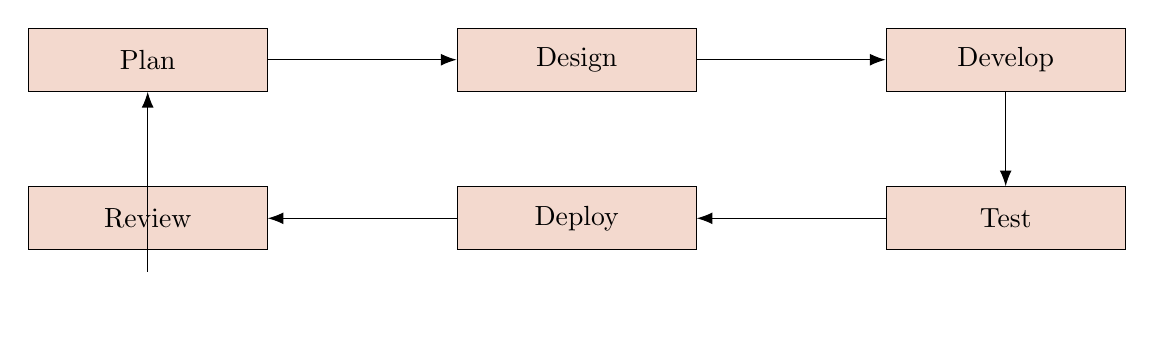
\begin{tikzpicture}[node distance=2.4cm]
  \node[process,fill=kmerwarm!20] (plan) {Plan};
  \node[process,fill=kmerwarm!20,right=of plan] (design) {Design};
  \node[process,fill=kmerwarm!20,right=of design] (develop) {Develop};
  \node[process,fill=kmerwarm!20,below=1.2cm of develop] (test) {Test};
  \node[process,fill=kmerwarm!20,left=of test] (deploy) {Deploy};
  \node[process,fill=kmerwarm!20,left=of deploy] (review) {Review};
  \draw[flow] (plan)--(design);
  \draw[flow] (design)--(develop);
  \draw[flow] (develop)--(test);
  \draw[flow] (test)--(deploy);
  \draw[flow] (deploy)--(review);
  \draw[flow] (review.south) .. controls +(0,-1) and +(0,-1) .. (plan.south);
\end{tikzpicture}
\caption{Agile Methodology}
\label{fig:agile}
\end{figure}

\subsection{Other Methodologies (Considered but Not Used)}
\subsubsection{Waterfall Model}
A linear model (Figure~\ref{fig:waterfall}) where each phase must complete before the next;
not chosen due to its rigidity and late feedback.

\begin{figure}[H]
\centering
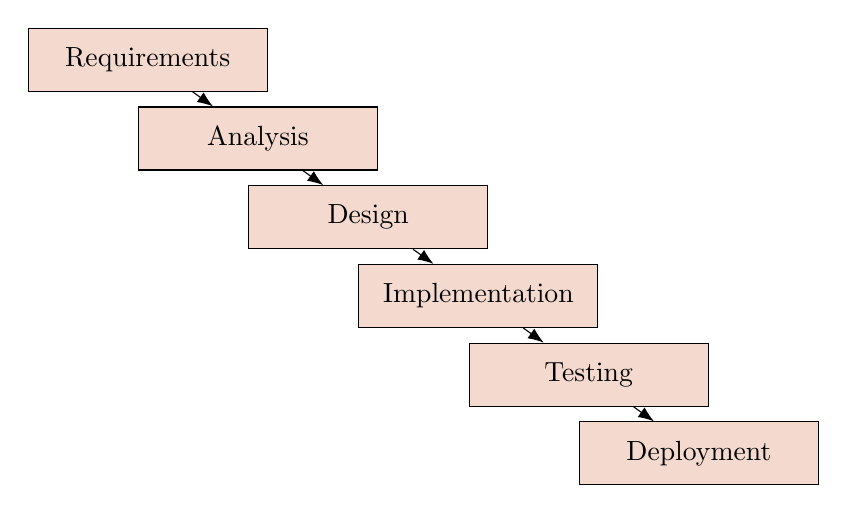
\begin{tikzpicture}[every node/.style={process,fill=kmerwarm!20,minimum width=2.6cm}]
  \node (r) at (0,0) {Requirements};
  \node (a) at (1.4,-1) {Analysis};
  \node (d) at (2.8,-2) {Design};
  \node (i) at (4.2,-3) {Implementation};
  \node (t) at (5.6,-4) {Testing};
  \node (dep) at (7.0,-5) {Deployment};
  \draw[flow] (r)--(a); \draw[flow] (a)--(d); \draw[flow] (d)--(i);
  \draw[flow] (i)--(t); \draw[flow] (t)--(dep);
\end{tikzpicture}
\caption{Waterfall Model}
\label{fig:waterfall}
\end{figure}

\subsubsection{V-Shape Model}
Pairs each development stage with a testing stage (Figure~\ref{fig:vmodel}); not chosen due
to rigidity and late user involvement.

\begin{figure}[H]
\centering
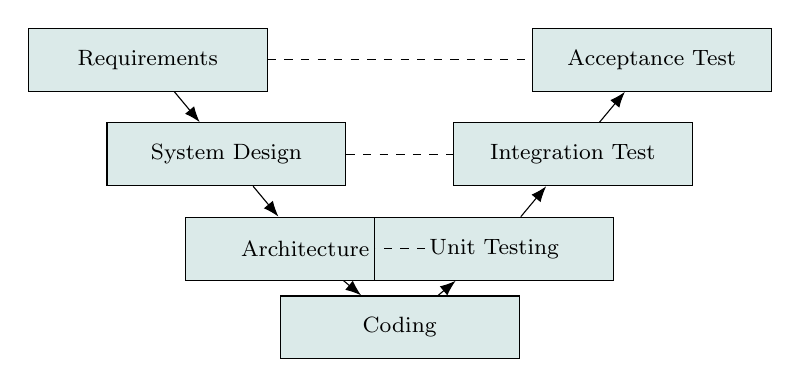
\begin{tikzpicture}[every node/.style={process,fill=kmerteal!15,minimum width=2.6cm,font=\footnotesize}]
  \node (req) at (0,0) {Requirements};
  \node (sys) at (1,-1.2) {System Design};
  \node (arch) at (2,-2.4) {Architecture};
  \node (code) at (3.2,-3.4) {Coding};
  \node (unit) at (4.4,-2.4) {Unit Testing};
  \node (integ) at (5.4,-1.2) {Integration Test};
  \node (acc) at (6.4,0) {Acceptance Test};
  \draw[flow] (req)--(sys); \draw[flow] (sys)--(arch); \draw[flow] (arch)--(code);
  \draw[flow] (code)--(unit); \draw[flow] (unit)--(integ); \draw[flow] (integ)--(acc);
  \draw[dashed] (req)--(acc); \draw[dashed] (sys)--(integ); \draw[dashed] (arch)--(unit);
\end{tikzpicture}
\caption{V-Shape Model (Verification and Validation)}
\label{fig:vmodel}
\end{figure}

\subsubsection{Spiral Model}
Combines iterative development with risk analysis; not ideal here due to complexity and
overhead. \emph{(A standard illustrative diagram of the Spiral Model can be inserted below.)}

\begin{figure}[H]
\screenshot{Diagramme du mod\`ele en spirale (Spiral Model) --- image illustrative \`a ins\'erer (\texttt{spiral.png}).}
\caption{Spiral Model}
\label{fig:spiral}
\end{figure}

\section{The System Architecture (MVC)}
K-MER EVENT follows the MVC pattern (Figure~\ref{fig:mvc}). The \textbf{Model} (Sequelize +
MySQL) holds users, events, bookings, carts and waitlist entries. The \textbf{View} (React +
Tailwind SPA) renders the interface. The \textbf{Controller} (Express routes/controllers)
handles requests, applies business rules, and emits real-time events via Socket.IO.

\begin{figure}[H]
\centering
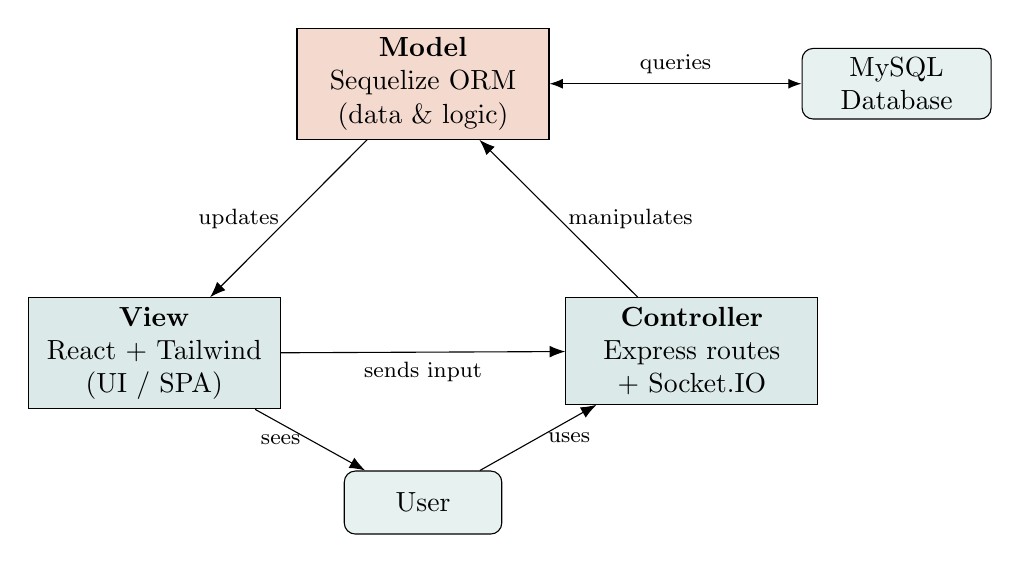
\begin{tikzpicture}[node distance=2.2cm and 2.6cm]
  \node[process,fill=kmerwarm!20,minimum width=3.2cm] (model) {\textbf{Model}\\Sequelize ORM\\(data \& logic)};
  \node[startstop,right=3.2cm of model,minimum width=2.4cm] (db) {MySQL\\Database};
  \node[process,fill=kmerteal!15,below left=2cm and 0.2cm of model,minimum width=3.2cm] (view) {\textbf{View}\\React + Tailwind\\(UI / SPA)};
  \node[process,fill=kmerteal!15,below right=2cm and 0.2cm of model,minimum width=3.2cm] (ctrl) {\textbf{Controller}\\Express routes\\+ Socket.IO};
  \node[startstop,below=4.2cm of model,minimum width=2cm] (user) {User};
  \draw[{Latex}-{Latex}] (model)--(db) node[midway,above,font=\footnotesize]{queries};
  \draw[flow] (ctrl) -- node[midway,right,font=\footnotesize]{manipulates} (model);
  \draw[flow] (model) -- node[midway,left,font=\footnotesize]{updates} (view);
  \draw[flow] (view) -- node[midway,below,font=\footnotesize,sloped]{sends input} (ctrl);
  \draw[flow] (view) -- node[midway,left,font=\footnotesize]{sees} (user);
  \draw[flow] (user) -- node[midway,right,font=\footnotesize]{uses} (ctrl);
\end{tikzpicture}
\caption{MVC Architecture Pattern adapted to K-MER EVENT}
\label{fig:mvc}
\end{figure}

\section{Project Planning and Scheduling}
Table~\ref{tab:plan} summarizes the project plan.

\begin{table}[h]
\centering
\caption{K-MER EVENT Project Plan}
\label{tab:plan}
\begin{tabular}{>{\raggedright}p{3cm}>{\raggedright}p{6cm}p{2cm}}
\toprule
\textbf{Phase} & \textbf{Description} & \textbf{Timeline}\\
\midrule
Project Initiation & Goals, roles, scope, tooling setup & Week 1\\
Requirements & Surveys, market research, user stories & Week 1--2\\
System Design & Architecture, wireframes, DB schema & Week 2\\
Development & Iterative sprints (frontend + backend) & Week 3--7\\
Testing \& QA & Unit, integration, system, UAT & Week 8\\
Deployment & VPS + Nginx + HTTPS, launch & Week 8\\
Maintenance & Monitoring, updates & Week 9\arraybackslash\\
\bottomrule
\end{tabular}
\end{table}

\section{Tools and Technologies}
\subsection{Hardware Tools}
A development workstation (Intel Core i5 / AMD Ryzen 5 or higher, 16 GB RAM, SSD), a range of
Android/iOS devices for responsive testing, and an internet connection.

\subsection{Software Tools and Technologies}
\begin{itemize}
  \item \textbf{Frontend:} React 18, Vite, Tailwind CSS, React Router, Axios, Recharts,
        Framer Motion, lucide-react, html5-qrcode, Leaflet/react-leaflet, socket.io-client.
  \item \textbf{Backend:} Node.js, Express, Sequelize, MySQL, JWT, Multer, PDFKit, qrcode,
        helmet, express-rate-limit, Socket.IO, Nodemailer.
  \item \textbf{Design tools:} Figma (wireframes), StarUML (UML diagrams).
  \item \textbf{Testing:} manual functional testing, API testing (Postman), UAT.
  \item \textbf{Version control:} Git and GitHub.
  \item \textbf{Geolocation/maps:} OpenStreetMap Nominatim (geocoding), Esri World Imagery
        (satellite tiles).
  \item \textbf{Colour scheme \& fonts:} a teal primary with a warm terracotta/ocre accent,
        and clean sans-serif typography for readability in light and dark themes.
\end{itemize}

\section{Ethical Considerations}
Survey participants gave informed consent; data was anonymized and stored securely.
Passwords are hashed (bcrypt) and sensitive endpoints protected by role-based access control.
Care was taken to minimize bias in questionnaire design.

\section{Conclusion}
This chapter described the Agile methodology, MVC architecture, tools and ethical measures
used to build K-MER EVENT. The next chapter presents the analysis, design, implementation
and findings.

% ============================ CHAPTER 4 ==============================
\chapter{ANALYSIS, DESIGN, IMPLEMENTATION AND FINDINGS}

\section{Introduction}
This chapter translates the methodology into results: statistical analysis of the survey,
the functional and non-functional requirements, the system design (UML diagrams), and the
implementation (screens of the live application).

\section{Statistical Analysis}
\subsection{Analysis of Collected Data}
A survey was distributed to potential users (attendees and organizers) to evaluate the need
for, and acceptance of, K-MER EVENT.\\
\emph{NB : les figures ci-dessous correspondent aux r\'esultats de VOTRE sondage. Ins\'erez
vos captures Google Forms (ou exportez les graphiques) \`a la place des encadr\'es.}

% ---- 15 figures de sondage (captures à insérer) ----
\begin{figure}[H]\screenshot{Q1 --- Tranche d'\^age des participants (graphique camembert).}\caption{Survey Question 1 --- Age}\end{figure}
\begin{figure}[H]\screenshot{Q2 --- Genre des participants.}\caption{Survey Question 2 --- Gender}\end{figure}
\begin{figure}[H]\screenshot{Q3 --- R\^ole (attendee / organizer / admin).}\caption{Survey Question 3 --- Role}\end{figure}
\begin{figure}[H]\screenshot{Q4 --- \`A quelle fr\'equence assistez-vous \`a des \'ev\'enements ?}\caption{Survey Question 4 --- Attendance frequency}\end{figure}
\begin{figure}[H]\screenshot{Q5 --- Comment d\'ecouvrez-vous actuellement les \'ev\'enements ?}\caption{Survey Question 5 --- How attendees discover events}\end{figure}
\begin{figure}[H]\screenshot{Q6 --- Quels d\'efis rencontrez-vous pour trouver/acheter des billets ?}\caption{Survey Question 6 --- Challenges}\end{figure}
\begin{figure}[H]\screenshot{Q7 --- Importance des fonctionnalit\'es (note de 1 \`a 5).}\caption{Survey Question 7 --- Feature importance}\end{figure}
\begin{figure}[H]\screenshot{Q8 --- Fonctionnalit\'es les plus utiles (recherche, billets QR, carte, etc.).}\caption{Survey Question 8 --- Most useful features}\end{figure}
\begin{figure}[H]\screenshot{Q9 --- Informations essentielles sur la page d'un \'ev\'enement.}\caption{Survey Question 9 --- Essential event information}\end{figure}
\begin{figure}[H]\screenshot{Q10 --- Mode de partage pr\'ef\'er\'e (WhatsApp, lien, etc.).}\caption{Survey Question 10 --- Preferred sharing}\end{figure}
\begin{figure}[H]\screenshot{Q11 --- Importance de la billetterie QR s\'ecuris\'ee.}\caption{Survey Question 11 --- QR ticket security}\end{figure}
\begin{figure}[H]\screenshot{Q12 --- Mesures qui inspirent confiance (organisateurs v\'erifi\'es, etc.).}\caption{Survey Question 12 --- Trust measures}\end{figure}
\begin{figure}[H]\screenshot{Q13 --- Moyen de paiement pr\'ef\'er\'e (Mobile Money, etc.).}\caption{Survey Question 13 --- Preferred payment}\end{figure}
\begin{figure}[H]\screenshot{Q14 --- Perception du prix des billets.}\caption{Survey Question 14 --- Ticket pricing}\end{figure}
\begin{figure}[H]\screenshot{Q15 --- Fr\'equence d'utilisation pr\'evue de l'application.}\caption{Survey Question 15 --- Intended usage frequency}\end{figure}

\subsection{Analysis of Requirements Gathered}
\subsubsection{Functional Requirements}
\begin{itemize}
  \item \textbf{Registration Module:} sign up, login, password recovery (JWT, bcrypt).
  \item \textbf{Profile Management:} attendee and organizer profiles with profile picture.
  \item \textbf{Event Discovery:} list of published events with banner, category, venue,
        city, date, price and remaining tickets.
  \item \textbf{Search and Filter:} by keyword, city, category, maximum price, upcoming and
        favorites.
  \item \textbf{Event Details:} photo gallery, optional video, satellite map, quantity
        selection, add to cart, favorite and WhatsApp share.
  \item \textbf{Cart and Checkout:} multi-event cart, attendee details, atomic stock
        decrement under a database transaction.
  \item \textbf{Ticketing:} downloadable PDF tickets with a unique QR code; ``My Tickets''
        with Active/Expired tabs.
  \item \textbf{Waitlist:} join the waitlist for a sold-out event; automatic e-mail when
        capacity increases.
  \item \textbf{QR Check-in:} camera scan or manual entry; detects valid / already used /
        cancelled / invalid; organizers limited to their own events.
  \item \textbf{Organizer:} create / edit / delete own events, capacity and price management,
        statistics (tickets sold, revenue, fill rate).
  \item \textbf{Admin:} analytics dashboard, event validation workflow (pending $\rightarrow$
        published), user CRUD, monitoring.
  \item \textbf{Real-time:} broadcast of event changes to all clients (Socket.IO).
  \item \textbf{Geolocation:} automatic geocoding from venue/city and a satellite map.
\end{itemize}

\subsubsection{Non-Functional Requirements}
\begin{itemize}
  \item \textbf{Performance:} responsive UI, low-latency API, caching of static assets.
  \item \textbf{Security:} hashed passwords, JWT, RBAC, helmet headers, rate limiting,
        tamper-proof QR tickets, \texttt{Cache-Control: no-store} on the API.
  \item \textbf{Usability:} intuitive, responsive interface with a readable light/dark theme.
  \item \textbf{Reliability:} high availability, regular database and uploads backups.
\end{itemize}

\section{Design}
\subsection{UML Diagrams}
UML diagrams visualize the structure and behaviour of K-MER EVENT: flowcharts, use-case,
class, ER and sequence diagrams.

\subsection{Flowchart Diagrams}
Figures~\ref{fig:flow-attendee}, \ref{fig:flow-org} and \ref{fig:flow-admin} show the
attendee, organizer and admin flows.

% ---- Attendee flowchart ----
\begin{figure}[H]
\centering
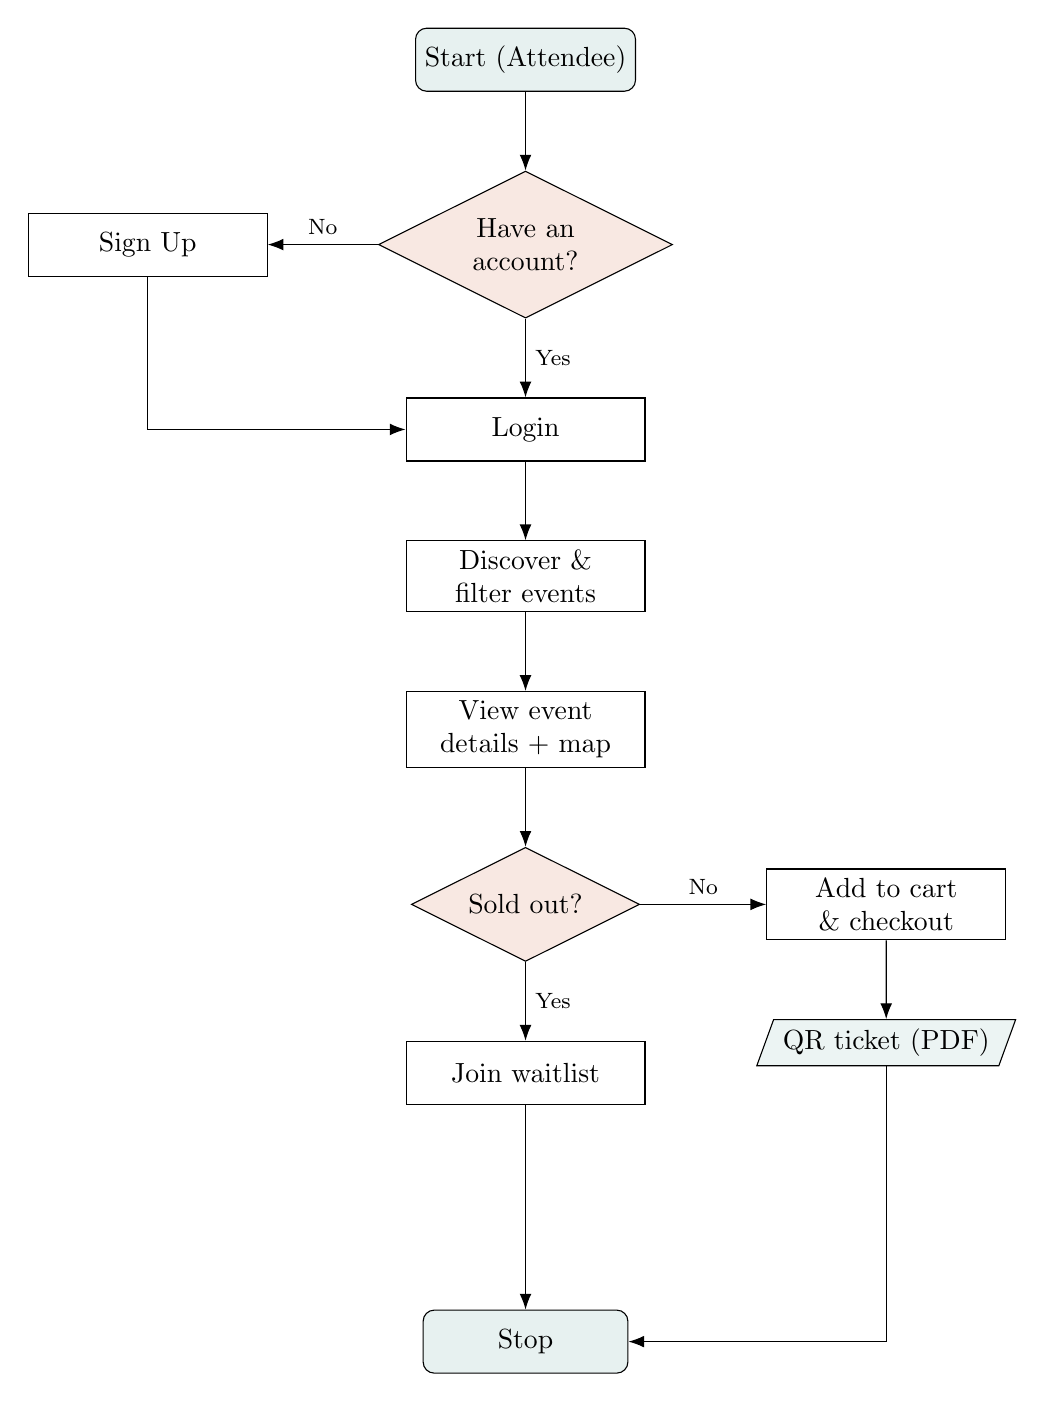
\begin{tikzpicture}[node distance=1.0cm and 1.4cm]
  \node[startstop] (start) {Start (Attendee)};
  \node[decision,below=of start] (acc) {Have an account?};
  \node[process,left=of acc] (signup) {Sign Up};
  \node[process,below=of acc] (login) {Login};
  \node[process,below=of login] (disc) {Discover \& filter events};
  \node[process,below=of disc] (details) {View event details + map};
  \node[decision,below=of details] (sold) {Sold out?};
  \node[process,right=1.6cm of sold] (cart) {Add to cart \& checkout};
  \node[process,below=of sold] (wait) {Join waitlist};
  \node[io,below=1.0cm of cart] (ticket) {QR ticket (PDF)};
  \node[startstop,below=2.6cm of wait] (stop) {Stop};
  \draw[flow] (start)--(acc);
  \draw[flow] (acc)-- node[above,font=\footnotesize]{No} (signup);
  \draw[flow] (signup)|-(login);
  \draw[flow] (acc)-- node[right,font=\footnotesize]{Yes} (login);
  \draw[flow] (login)--(disc);
  \draw[flow] (disc)--(details);
  \draw[flow] (details)--(sold);
  \draw[flow] (sold)-- node[above,font=\footnotesize]{No} (cart);
  \draw[flow] (sold)-- node[right,font=\footnotesize]{Yes} (wait);
  \draw[flow] (cart)--(ticket);
  \draw[flow] (ticket)|-(stop);
  \draw[flow] (wait)--(stop);
\end{tikzpicture}
\caption{Attendee Flow Chart}
\label{fig:flow-attendee}
\end{figure}

% ---- Organizer flowchart ----
\begin{figure}[H]
\centering
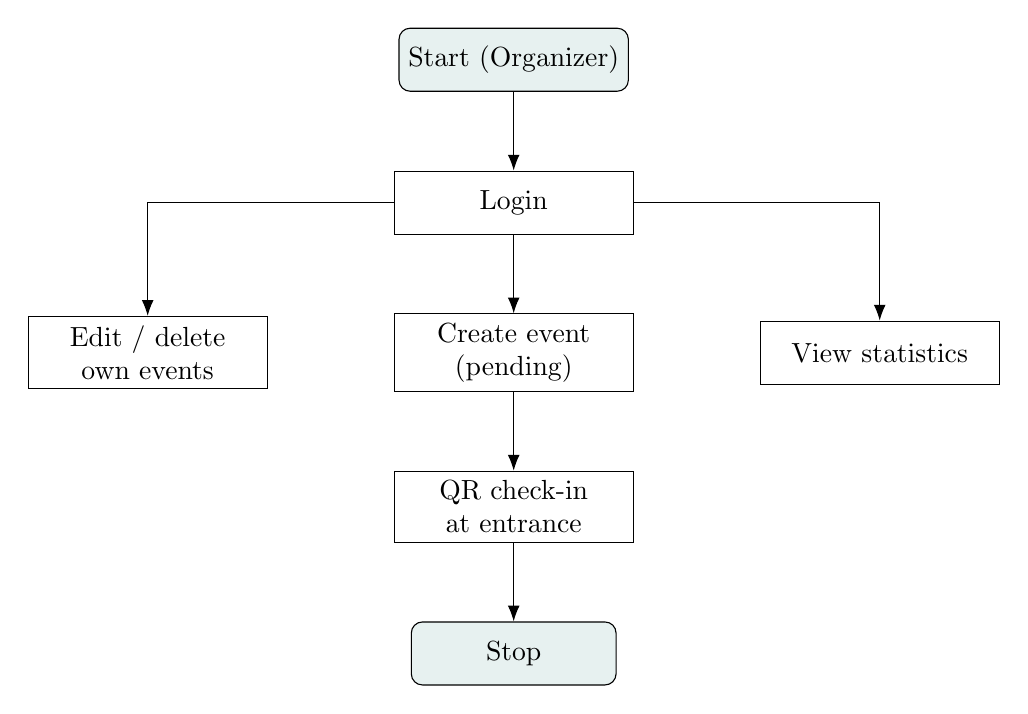
\begin{tikzpicture}[node distance=1.0cm and 1.2cm]
  \node[startstop] (start) {Start (Organizer)};
  \node[process,below=of start] (login) {Login};
  \node[process,below=of login] (create) {Create event (pending)};
  \node[process,left=1.6cm of create] (edit) {Edit / delete own events};
  \node[process,right=1.6cm of create] (stats) {View statistics};
  \node[process,below=of create] (checkin) {QR check-in at entrance};
  \node[startstop,below=of checkin] (stop) {Stop};
  \draw[flow] (start)--(login);
  \draw[flow] (login)--(create);
  \draw[flow] (login)-|(edit);
  \draw[flow] (login)-|(stats);
  \draw[flow] (create)--(checkin);
  \draw[flow] (checkin)--(stop);
\end{tikzpicture}
\caption{Organizer Flow Chart}
\label{fig:flow-org}
\end{figure}

% ---- Admin flowchart ----
\begin{figure}[H]
\centering
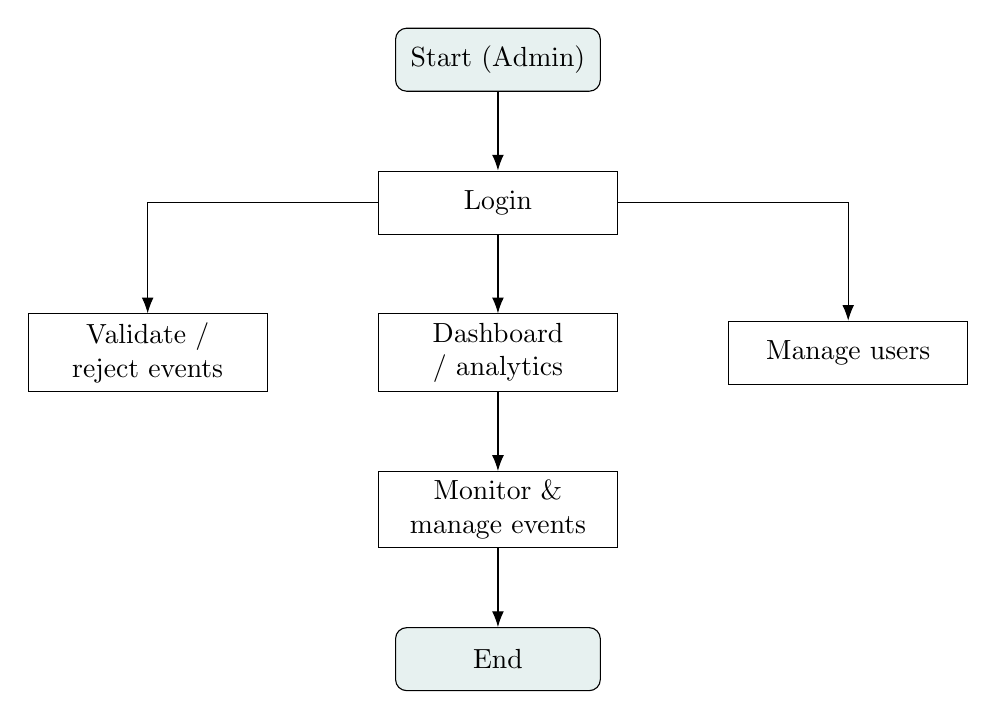
\begin{tikzpicture}[node distance=1.0cm and 0.9cm]
  \node[startstop] (start) {Start (Admin)};
  \node[process,below=of start] (login) {Login};
  \node[process,below=of login] (dash) {Dashboard / analytics};
  \node[process,left=1.4cm of dash] (validate) {Validate / reject events};
  \node[process,right=1.4cm of dash] (users) {Manage users};
  \node[process,below=of dash] (monitor) {Monitor \& manage events};
  \node[startstop,below=of monitor] (end) {End};
  \draw[flow] (start)--(login);
  \draw[flow] (login)--(dash);
  \draw[flow] (login)-|(validate);
  \draw[flow] (login)-|(users);
  \draw[flow] (dash)--(monitor);
  \draw[flow] (monitor)--(end);
\end{tikzpicture}
\caption{Admin Flow Chart}
\label{fig:flow-admin}
\end{figure}

\subsection{Use Case Diagram}
Figure~\ref{fig:usecase} shows the main use cases for the three actors.

\begin{figure}[H]
\centering
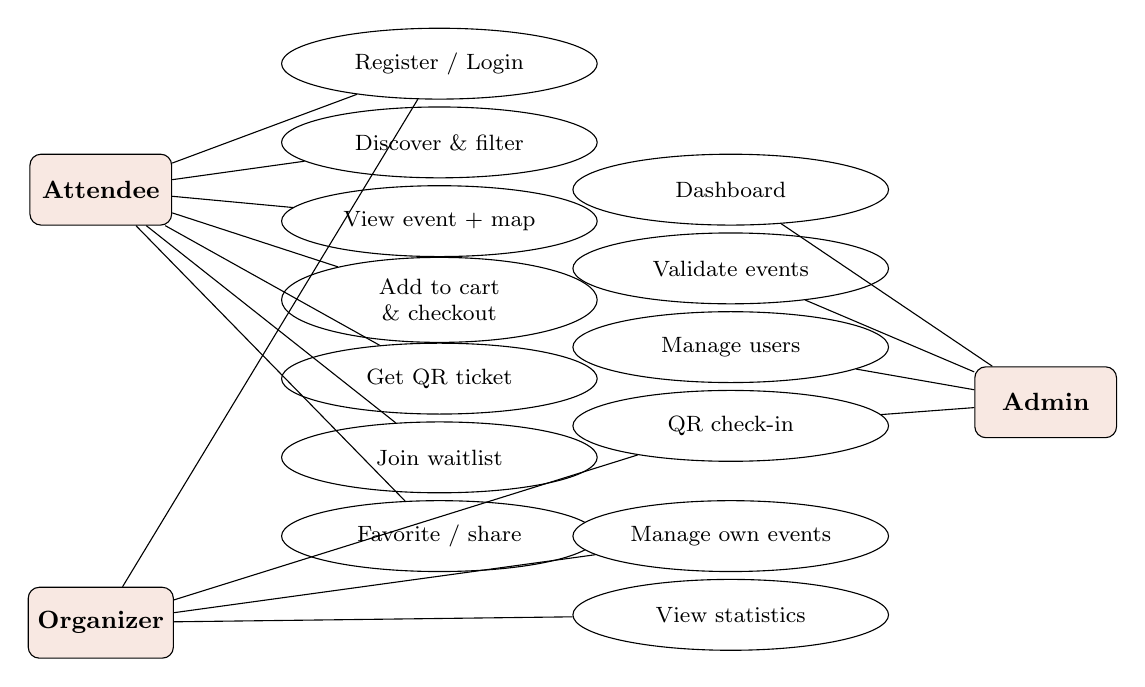
\begin{tikzpicture}[node distance=0.55cm]
  % actors
  \node[actor] (att) at (0,0) {Attendee};
  \node[actor] (org) at (0,-5.5) {Organizer};
  \node[actor] (adm) at (12,-2.7) {Admin};
  % use cases (attendee/organizer side)
  \node[uc] (u1) at (4.3,1.6) {Register / Login};
  \node[uc] (u2) at (4.3,0.6) {Discover \& filter};
  \node[uc] (u3) at (4.3,-0.4) {View event + map};
  \node[uc] (u4) at (4.3,-1.4) {Add to cart \& checkout};
  \node[uc] (u5) at (4.3,-2.4) {Get QR ticket};
  \node[uc] (u6) at (4.3,-3.4) {Join waitlist};
  \node[uc] (u7) at (4.3,-4.4) {Favorite / share};
  \node[uc] (o1) at (8,-4.4) {Manage own events};
  \node[uc] (o2) at (8,-5.4) {View statistics};
  \node[uc] (c1) at (8,-1.0) {Validate events};
  \node[uc] (c2) at (8,-2.0) {Manage users};
  \node[uc] (c3) at (8,-3.0) {QR check-in};
  \node[uc] (c4) at (8,0.0) {Dashboard};
  % links attendee
  \foreach \u in {u1,u2,u3,u4,u5,u6,u7} \draw (att)--(\u);
  % links organizer
  \foreach \u in {u1,o1,o2,c3} \draw (org)--(\u);
  % links admin
  \foreach \u in {c1,c2,c3,c4} \draw (adm)--(\u);
\end{tikzpicture}
\caption{K-MER EVENT Use Case Diagram}
\label{fig:usecase}
\end{figure}

\subsection{Class Diagram}
Figure~\ref{fig:class} shows the main classes and their relationships.

\begin{figure}[H]
\centering
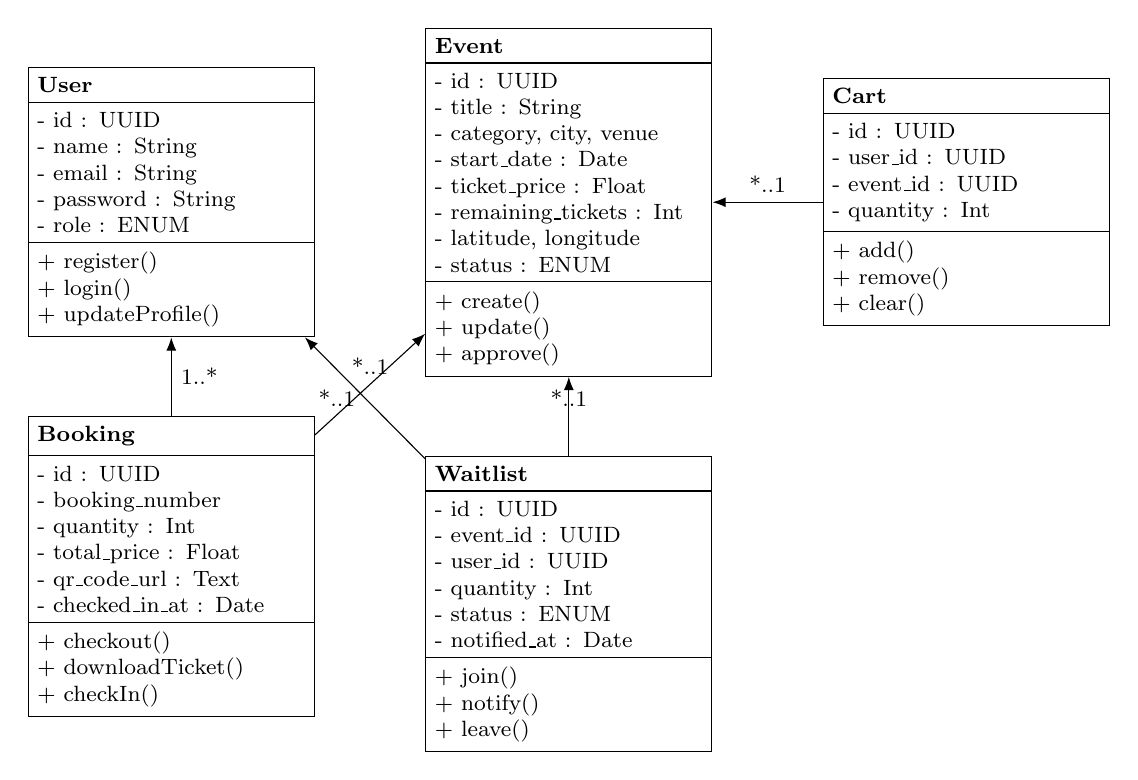
\begin{tikzpicture}[node distance=1.0cm and 1.4cm]
  \node[classbox] (user) {
    \textbf{User}
    \nodepart{second} - id : UUID\\ - name : String\\ - email : String\\ - password : String\\ - role : ENUM
    \nodepart{third} + register()\\ + login()\\ + updateProfile()};
  \node[classbox,right=of user] (event) {
    \textbf{Event}
    \nodepart{second} - id : UUID\\ - title : String\\ - category, city, venue\\ - start\_date : Date\\ - ticket\_price : Float\\ - remaining\_tickets : Int\\ - latitude, longitude\\ - status : ENUM
    \nodepart{third} + create()\\ + update()\\ + approve()};
  \node[classbox,below=of user] (booking) {
    \textbf{Booking}
    \nodepart{second} - id : UUID\\ - booking\_number\\ - quantity : Int\\ - total\_price : Float\\ - qr\_code\_url : Text\\ - checked\_in\_at : Date
    \nodepart{third} + checkout()\\ + downloadTicket()\\ + checkIn()};
  \node[classbox,below=of event] (waitlist) {
    \textbf{Waitlist}
    \nodepart{second} - id : UUID\\ - event\_id : UUID\\ - user\_id : UUID\\ - quantity : Int\\ - status : ENUM\\ - notified\_at : Date
    \nodepart{third} + join()\\ + notify()\\ + leave()};
  \node[classbox,right=of event] (cart) {
    \textbf{Cart}
    \nodepart{second} - id : UUID\\ - user\_id : UUID\\ - event\_id : UUID\\ - quantity : Int
    \nodepart{third} + add()\\ + remove()\\ + clear()};
  % relations
  \draw[-{Latex}] (booking) -- node[right,font=\footnotesize]{1..*} (user);
  \draw[-{Latex}] (booking) -- node[above,font=\footnotesize]{*..1} (event);
  \draw[-{Latex}] (waitlist) -- node[above,font=\footnotesize]{*..1} (event);
  \draw[-{Latex}] (waitlist) -- node[left,font=\footnotesize]{*..1} (user);
  \draw[-{Latex}] (cart) -- node[above,font=\footnotesize]{*..1} (event);
\end{tikzpicture}
\caption{Class Diagram}
\label{fig:class}
\end{figure}

\subsection{ER Diagram}
Figure~\ref{fig:er} shows the database entities and their relationships.\\
\emph{NB : vous pouvez aussi g\'en\'erer un sch\'ema d\'etaill\'e depuis phpMyAdmin / MySQL
Workbench et l'ins\'erer \`a la place.}

\begin{figure}[H]
\centering
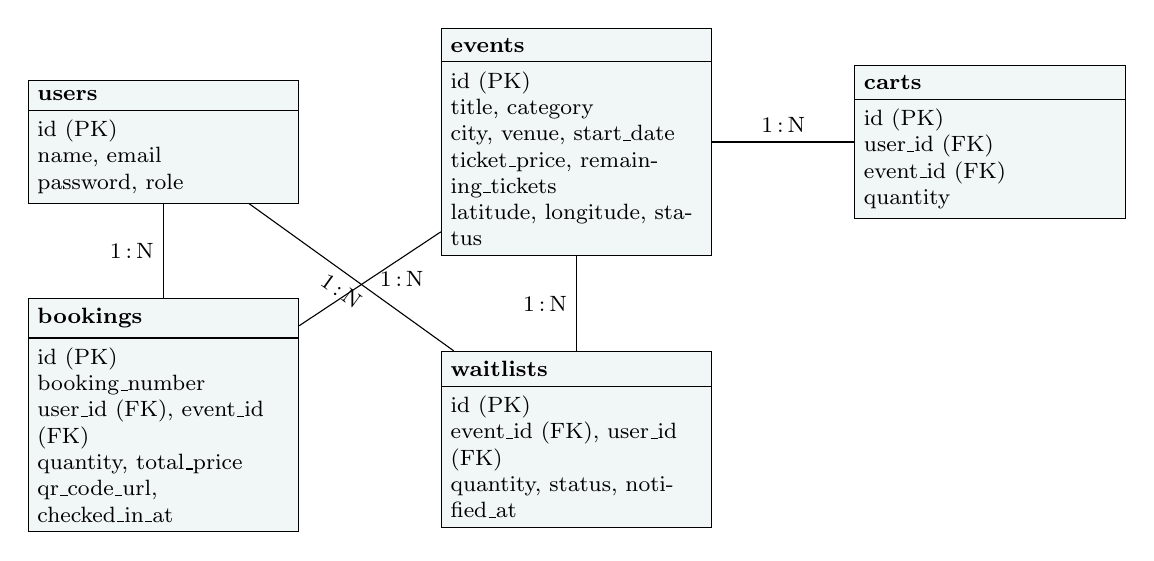
\begin{tikzpicture}[node distance=1.2cm and 1.8cm]
  \node[entity] (users) {\textbf{users}\nodepart{second}id (PK)\\name, email\\password, role};
  \node[entity,right=of users] (events) {\textbf{events}\nodepart{second}id (PK)\\title, category\\city, venue, start\_date\\ticket\_price, remaining\_tickets\\latitude, longitude, status};
  \node[entity,below=of users] (bookings) {\textbf{bookings}\nodepart{second}id (PK)\\booking\_number\\user\_id (FK), event\_id (FK)\\quantity, total\_price\\qr\_code\_url, checked\_in\_at};
  \node[entity,below=of events] (waitlists) {\textbf{waitlists}\nodepart{second}id (PK)\\event\_id (FK), user\_id (FK)\\quantity, status, notified\_at};
  \node[entity,right=of events] (carts) {\textbf{carts}\nodepart{second}id (PK)\\user\_id (FK)\\event\_id (FK)\\quantity};
  \draw (users) -- node[left,font=\footnotesize]{1\,:\,N} (bookings);
  \draw (events) -- node[right,font=\footnotesize]{1\,:\,N} (bookings);
  \draw (events) -- node[left,font=\footnotesize]{1\,:\,N} (waitlists);
  \draw (users) -- node[below,font=\footnotesize,sloped]{1\,:\,N} (waitlists);
  \draw (events) -- node[above,font=\footnotesize]{1\,:\,N} (carts);
\end{tikzpicture}
\caption{ER Diagram}
\label{fig:er}
\end{figure}

\subsection{Sequence Diagrams}
Figures~\ref{fig:seq-booking}, \ref{fig:seq-waitlist} and \ref{fig:seq-checkin} show three
key interactions.

% ---- Sequence: booking + QR ticket ----
\begin{figure}[H]
\centering
\resizebox{0.95\textwidth}{!}{%
\begin{sequencediagram}
  \newthread{a}{Attendee}
  \newinst[2]{s}{System (API)}
  \newinst[2]{db}{Database}
  \begin{call}{a}{Login}{s}{Dashboard}\end{call}
  \begin{call}{a}{Discover \& select event}{s}{Event details}
    \begin{call}{s}{Query event}{db}{Event data}\end{call}
  \end{call}
  \begin{call}{a}{Add to cart \& checkout}{s}{Confirmation}
    \begin{call}{s}{Decrement stock (transaction)}{db}{OK}\end{call}
    \begin{call}{s}{Create booking + QR}{db}{Saved}\end{call}
  \end{call}
  \mess{s}{Return PDF QR ticket}{a}
\end{sequencediagram}}
\caption{Sequence Diagram --- Booking and QR Ticket Generation}
\label{fig:seq-booking}
\end{figure}

% ---- Sequence: waitlist + notification ----
\begin{figure}[H]
\centering
\resizebox{0.95\textwidth}{!}{%
\begin{sequencediagram}
  \newthread{a}{Attendee}
  \newinst[2]{s}{System (API)}
  \newinst[2]{db}{Database}
  \newinst[2]{m}{Mail Service}
  \begin{call}{a}{Join waitlist (sold-out event)}{s}{Confirmation}
    \begin{call}{s}{Save waitlist entry}{db}{Saved}\end{call}
  \end{call}
  \begin{sdblock}{Capacity increases}{Organizer raises capacity}
    \begin{call}{s}{Find waiting users}{db}{List}\end{call}
    \begin{call}{s}{Send availability e-mail}{m}{Sent}\end{call}
    \mess{s}{Mark as notified}{db}
  \end{sdblock}
\end{sequencediagram}}
\caption{Sequence Diagram --- Waitlist and Notification}
\label{fig:seq-waitlist}
\end{figure}

% ---- Sequence: QR check-in ----
\begin{figure}[H]
\centering
\resizebox{0.95\textwidth}{!}{%
\begin{sequencediagram}
  \newthread{o}{Organizer/Admin}
  \newinst[2]{s}{System (API)}
  \newinst[2]{db}{Database}
  \begin{call}{o}{Scan QR / enter code}{s}{Result}
    \begin{call}{s}{Find booking}{db}{Booking}\end{call}
    \begin{sdblock}{Validation}{check status \& ownership}
      \mess{s}{Set checked\_in\_at}{db}
    \end{sdblock}
  \end{call}
  \mess{s}{Valid / Already used / Invalid}{o}
\end{sequencediagram}}
\caption{Sequence Diagram --- QR Check-in at the Entrance}
\label{fig:seq-checkin}
\end{figure}

\section{Implementation}
The implementation translated the design into a working React SPA and an Express REST API.
The screens below show the live application.\\
\emph{NB : remplacez chaque encadr\'e par une CAPTURE D'\'ECRAN de votre application
(\texttt{.png}).}

\begin{figure}[H]\screenshot{Page d'accueil / d\'ecouverte (Discover) avec recherche et filtres.}\caption{Home / Discover Page}\end{figure}
\begin{figure}[H]\screenshot{Page de connexion (Login).}\caption{Login Page}\end{figure}
\begin{figure}[H]\screenshot{Inscription utilisateur / organisateur (Register).}\caption{User and Organizer Registration}\end{figure}
\begin{figure}[H]\screenshot{Liste des \'ev\'enements (cartes : banni\`ere, cat\'egorie, lieu, prix, places).}\caption{Events Listing Page}\end{figure}
\begin{figure}[H]\screenshot{Page d\'etail d'un \'ev\'enement : galerie, vid\'eo, carte satellite, quantit\'e.}\caption{Event Details Page (with satellite map)}\end{figure}
\begin{figure}[H]\screenshot{Panier (Cart) et page de paiement (Checkout).}\caption{Cart and Checkout}\end{figure}
\begin{figure}[H]\screenshot{Billet PDF avec QR code g\'en\'er\'e apr\`es r\'eservation.}\caption{PDF Ticket with QR Code}\end{figure}
\begin{figure}[H]\screenshot{Mes billets (onglets Actifs / Expir\'es) + section Liste d'attente.}\caption{My Tickets and Waitlist}\end{figure}
\begin{figure}[H]\screenshot{Page de check-in QR (cam\'era + saisie manuelle).}\caption{QR Check-in Page}\end{figure}
\begin{figure}[H]\screenshot{Tableau de bord organisateur (cr\'eation/\'edition + statistiques).}\caption{Organizer Dashboard}\end{figure}
\begin{figure}[H]\screenshot{Tableau de bord administrateur (analytics, validation, utilisateurs).}\caption{Admin Dashboard}\end{figure}

This chapter showed that K-MER EVENT was designed with a user-centric, systematic approach,
using UML diagrams to capture both the static and dynamic aspects of the system and ensuring
a smooth transition from design to implementation.

% ============================ CHAPTER 5 ==============================
\chapter{SUMMARY, CONCLUSIONS, DISCUSSION, AND RECOMMENDATIONS}

\section{Introduction}
This chapter summarizes the findings, draws conclusions, discusses implications and offers
recommendations for practice and further study.

\section{Summary}
The objective of this study was to streamline event discovery and ticketing through the
development of K-MER EVENT. The research explored existing ticketing platforms, gathered user
requirements through surveys, and designed, built and tested the application. Key insights:
\begin{enumerate}
  \item \textbf{Insecure, informal ticketing} causes fraud and access-control problems.
  \item \textbf{Users prefer} a single platform with search/filters, secure QR tickets,
        clear locations and real-time availability.
  \item \textbf{Agile development} with React, Node/Express, Sequelize/MySQL and Socket.IO
        delivered a real-time, role-based platform with QR ticketing, waitlist and maps.
\end{enumerate}

\section{Conclusions}
\begin{enumerate}
  \item \textbf{Streamlined process:} K-MER EVENT simplifies discovery, booking and
        ticketing, with favorites, sharing and a satellite-map location.
  \item \textbf{Secure access control:} unique QR tickets and QR check-in prevent forgery and
        speed up entry.
  \item \textbf{Real-time and engaging:} live updates and an automatic waitlist keep
        attendees informed and capture demand for sold-out events.
\end{enumerate}

\section{Discussion}
The results indicate that K-MER EVENT effectively addresses key problems in the local event
industry by digitizing and securing ticketing. By allowing attendees to filter events by
city, category, price and date, and to see the exact venue on a satellite map, the platform
makes participation more convenient and trustworthy. Real-time updates and QR check-in
improve both the attendee and organizer experience. Challenges remain in payment integration
and ensuring connectivity for all users.

\section{Recommendations for Practice}
\begin{enumerate}
  \item \textbf{Mobile Money integration:} add MTN Mobile Money and Orange Money for in-app
        ticket payment.
  \item \textbf{Native mobile app:} build Android/iOS apps for offline tickets and push
        notifications.
  \item \textbf{Organizer verification:} add a verification/badge system to build trust.
  \item \textbf{User testing:} conduct broader UAT to refine the experience.
  \item \textbf{Awareness and adoption:} run targeted marketing toward organizers and
        attendees.
\end{enumerate}

\section{For Further Study}
\begin{enumerate}
  \item \textbf{Longitudinal study} of platform impact on event attendance over time.
  \item \textbf{Partnerships} with venues, promoters and institutions to integrate official
        ticketing.
\end{enumerate}

% ============================ REFERENCES ==============================
\begin{thebibliography}{99}
\addcontentsline{toc}{chapter}{References}
\bibitem{eventbrite} Eventbrite Inc. (2023). \emph{How online ticketing works}. Eventbrite Help Center.
\bibitem{socketio} Socket.IO. (2024). \emph{Bidirectional and low-latency communication for every platform}. \url{https://socket.io}
\bibitem{express} OpenJS Foundation. (2024). \emph{Express --- Fast, unopinionated, minimalist web framework for Node.js}. \url{https://expressjs.com}
\bibitem{react} Meta Open Source. (2024). \emph{React --- A JavaScript library for building user interfaces}. \url{https://react.dev}
\bibitem{sequelize} Sequelize. (2024). \emph{Sequelize ORM documentation}. \url{https://sequelize.org}
\bibitem{mysql} Oracle. (2023). \emph{MySQL 8.0 Reference Manual}. Oracle Corporation.
\bibitem{jwt} Jones, M., Bradley, J., \& Sakimura, N. (2015). \emph{JSON Web Token (JWT), RFC 7519}. IETF.
\bibitem{osm} OpenStreetMap Foundation. (2024). \emph{Nominatim geocoding service}. \url{https://nominatim.org}
\bibitem{leaflet} Agafonkin, V. (2024). \emph{Leaflet --- an open-source JavaScript library for mobile-friendly interactive maps}. \url{https://leafletjs.com}
\bibitem{momo} GSMA. (2024). \emph{The State of the Industry Report on Mobile Money}. \url{https://www.gsma.com/mobilemoney}
\bibitem{agile} Beck, K. et al. (2001). \emph{Manifesto for Agile Software Development}. \url{https://agilemanifesto.org}
\bibitem{qr} ISO/IEC 18004:2015. \emph{Information technology --- Automatic identification and data capture techniques --- QR Code bar code symbology specification}.
\bibitem{owasp} OWASP Foundation. (2021). \emph{OWASP Top Ten Web Application Security Risks}. \url{https://owasp.org/Top10}
\end{thebibliography}

% ============================ APPENDIX ==============================
\chapter*{Appendix}
\addcontentsline{toc}{chapter}{Appendix}
\noindent\textbf{Survey Form for K-MER EVENT}\\
\texttt{[Lien Google Forms de votre sondage]}

\vspace{0.4cm}
\noindent\textbf{GitHub Repository}\\
\url{https://github.com/NLP1703/k-mer-event}

\end{document}
